\chapter{Конструкторский раздел}
В конструкторской части разработано программное обеспечение, а также формально описаны применяемые алгоритмы.

\section{Описание структур данных}
!!!!
\section{Общий алгоритм }
\section{Схемы алгоритм визуализации трехмерной схемы}
\subsection{Алгоритм z-буффер}
На рисунке~\ref{fig:z_buf} представлена схема алгоритма z-буфера.
\begin{figure}[H]
	\centering
	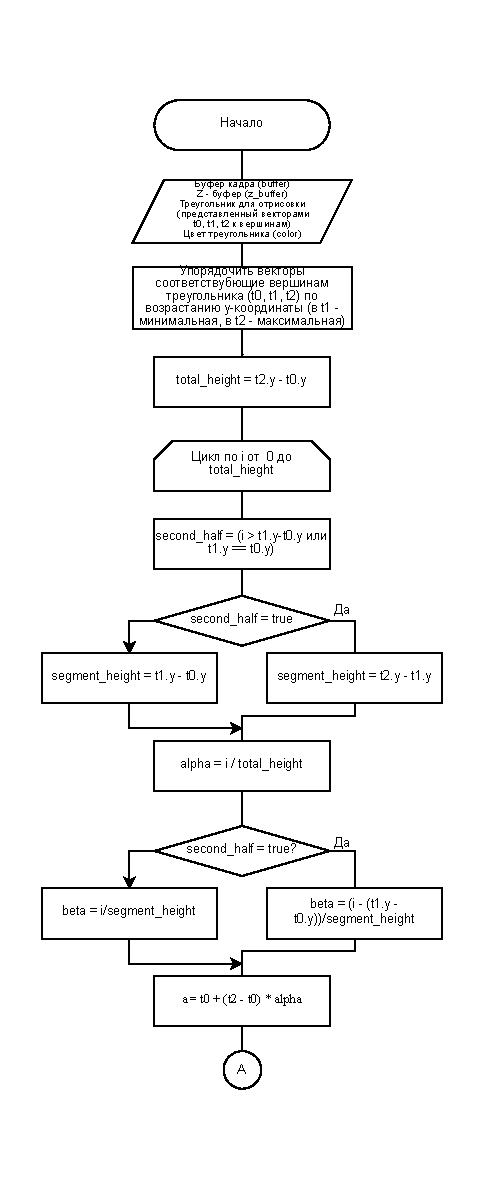
\includegraphics[width=0.6\textwidth, page=1]{assets/img/z-bufer.pdf}   
	\caption{Схема алгоритма z-буфера}
	\label{fig:z_buf}
\end{figure}

\subsection{Алгоритм поведения газов}

На рисунке~\ref{fig:Navie-Stocks} представлена схема алгоритма поведения газа на основе уравнений Навье---Стокса. 
\begin{figure}[H]
	\centering
	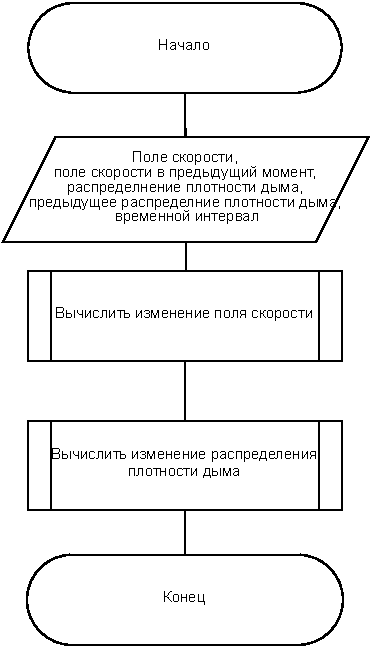
\includegraphics[width=0.7\textwidth, page=1]{assets/img/Naive_stocks.pdf}   
	\caption{Схема алгоритма на основе уравнения Навье---Стокса}
	\label{fig:Navie-Stocks}
\end{figure}

На рисунке~\ref{fig:dens_step} представлена схема алгоритма обновления распределения плотности.

\section*{Вывод}
В разделе спроектировано разрабатываемое программное обеспечение для визуализации сакуры, качающейся на ветру, приведены схемы алгоритмов.
